%%%%%%%%%%%%%%%%%%%%%%%%%%%%%%%%%%%%%%%%%%%%%%%%%%%%%%%%%%%%%%%%%%%%%%%%%%%

\documentclass[a4paper,oneside,12pt]{article}
\usepackage{mystyle}

\begin{document}

\title{\Large\bf Approximate $\pi$}
\author{%%
  Minh Van Nguyen \\
  \url{mvngu@gmx.com}
}
\date{\today}
\maketitle


%%%%%%%%%%%%%%%%%%%%%%%%%%%%%%%%%%%%%%%%%%%%%%%%%%%%%%%%%%%%%%%%%%%%%%%%%%%

\section{The number $\pi$}

The number $\pi = 3.141592\dots$ is another example of an irrational
number.  The number $\pi$ is often used to measure the area and
circumference of a circle; see \Figure{fig:general_circle}.  Since
$\pi$ is irrational, the number cannot be written as a ratio of
integers.  So for practical purposes, you must approximate $\pi$ as
closely as you can.  The Greek mathematician Archimedes used the
fraction $22 / 7$ to approximate $\pi$.  The fraction $22 / 7$ can be
written as $22 / 7 \approx 3.142857$, correct to six decimal digits.
(The symbol ``$\approx$'' means ``approximately''.)  This is not a
good approximation of $\pi$ because the value of $22 / 7$ differs from
$\pi$ from the third decimal digit onwards.  If a number $p \in \RR$
is to be a good approximation of $\pi$, then it should be possible to
make $p$ as close to $\pi$ as you want.

\begin{figure}[!htbp]
\centering
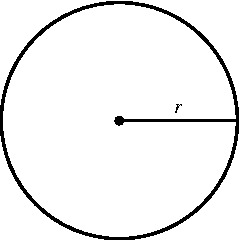
\includegraphics[scale=1]{image/05/circle.pdf}
\caption{%%
  A circle with radius $r$.  Since the radius cannot be negative, you
  must have $r \geq 0$.  The \emph{radius} of a circle is defined as
  the distance from the centre of the circle to any point on the
  circle.  The \emph{diameter}, denoted $d$, is then defined as twice
  the radius, i.e.~$d = 2r$.  The distance around the circle is called
  its \emph{circumference}.
}
\label{fig:general_circle}
\end{figure}

In order to approximate $\pi$ as closely as possible, you must know
how $\pi$ is defined.  Let $c$ be the circumference of a circle and
let $d$ be the diameter of the same circle.  Then the value of $\pi$
is defined as the ratio
%%
\begin{equation}
\label{eqn:define_pi_as_ratio_of_c_over_d}
\pi
=
\frac{c}{d}.
\end{equation}
%%
You already know that the diameter is equal to twice the radius.  The
only problem now is:
%%
\begin{packeditem}
\item How do you calculate the value of the circumference $c$?
\end{packeditem}
%%
The short answer is: You approximate the value of $c$ and then
substitute the values of $c$ and $d$ into
\Equation{eqn:define_pi_as_ratio_of_c_over_d} to obtain an
approximation of $\pi$.  What follows is the long answer.

\begin{exercise}
Describe the circle whose radius is zero.
\end{exercise}

\ifbool{showSolution}{
\begin{solution}
The circle whose radius is zero is an infinitely small point.
\end{solution}
}{}


%%%%%%%%%%%%%%%%%%%%%%%%%%%%%%%%%%%%%%%%%%%%%%%%%%%%%%%%%%%%%%%%%%%%%%%%%%%

\section{Approximating $\pi$ with a square}

Let's start by approximating the value of $\pi$ with a square.  The
square is drawn inside a unit circle such that the four corners of the
square touch the circle; see \Figure{fig:circle_inscribed_square}.
Since the unit circle has a radius of $1$, then the unit circle has a
diameter of $d = 2$.  What remains is to approximate the circumference
$c$ of the unit circle.

\begin{figure}[!htbp]
\centering
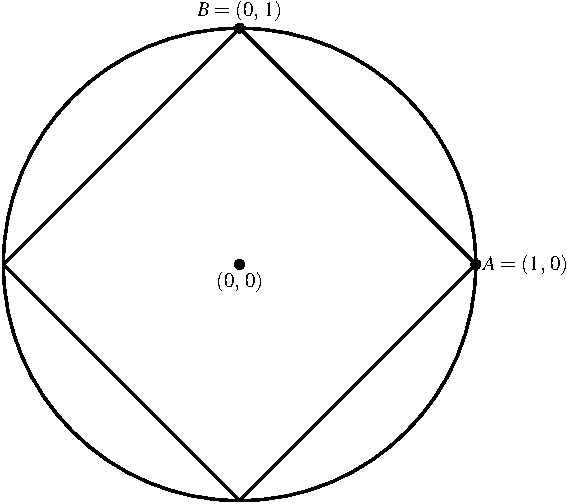
\includegraphics[scale=1.1]{image/05/circle-square.pdf}
\caption{%%
  A unit circle with an inscribed square.  A \emph{unit circle} is a
  circle whose radius is $1$.  The centre of the circle has
  coordinates $\tuple{0}{0}$.  The points $\quadruple{A}{B}{C}{D}$ are
  where the square touches the circle.  Any two neighbouring points
  are $\degree{90}$~(or $\pi / 2$ radians) apart.
}
\label{fig:circle_inscribed_square}
\end{figure}

\Figure{fig:circle_inscribed_square} suggests that the circumference
of the unit circle can be approximated by the perimeter of the
inscribed square.  If a square has a side length of $\ell$, then the
perimeter of the square is the sum of all the four sides of the
square.  In other words, the square has a perimeter of
$4\ell = \ell + \ell + \ell + \ell$.  For the square in
\Figure{fig:circle_inscribed_square} the value of $\ell$ is the length
of the line segment $AB$, which can be calculated as
%%
\begin{align*}
\ell
&=
\sqrt{(0 - 1)^2 + (1 - 0)^2} \\[4pt]
&=
\sqrt{1 + 1} \\[4pt]
&=
\sqrt{2}.
\end{align*}
%%
So the square has a perimeter of $4\ell = 4\sqrt{2}$ and you can take
this value to be an approximation of the circumference of the unit
circle.  Using \Equation{eqn:define_pi_as_ratio_of_c_over_d} you see
that the value of $\pi$ can be approximated as
%%
\begin{equation}
\label{eqn:approximate_pi_inscribed_square}
\begin{aligned}
\pi
&\approx
\frac{4\sqrt{2}}{2} \\[4pt]
&\approx
2\sqrt{2} \\[4pt]
&\approx
2.828427
\end{aligned}
\end{equation}
%%
correct to six decimal places.  The approximation of $2\sqrt{2}$ is
worst than Archimedes' approximate value of $22/7$.  Is there a way to
get a better approximation of $\pi$?

\begin{exercise}
Determine the area of the unit circle.
\end{exercise}

\ifbool{showSolution}{
\begin{solution}
If $r$ is the radius of a circle, then the circle has an area of
$\pi r^2$.  The unit circle has a radius of $r = 1$ so the area of the
unit circle is $\pi \times 1^2 = \pi$.
\end{solution}
}{}

\begin{exercise}
Calculate the area of the square in
\Figure{fig:circle_inscribed_square}.
\end{exercise}

\ifbool{showSolution}{
\begin{solution}
If $w$ is the width of a square, then the square has an area of
$w^2$.  As the square in \Figure{fig:circle_inscribed_square} has a
width of $\sqrt{2}$, the area of the square is $(\sqrt{2})^2 = 2$.
\end{solution}
}{}


%%%%%%%%%%%%%%%%%%%%%%%%%%%%%%%%%%%%%%%%%%%%%%%%%%%%%%%%%%%%%%%%%%%%%%%%%%%

\section{Approximate $\pi$ with an octagon}

Any two neighbouring corners of the square in
\Figure{fig:circle_inscribed_square} are separated by $\pi / 2$
radians.  If you decrease the angle that separates two neighbouring
corners, then you would expect to get a better approximation to the
value of $\pi$.  Let's put the above strategy into practice.

\begin{figure}[!htbp]
\centering
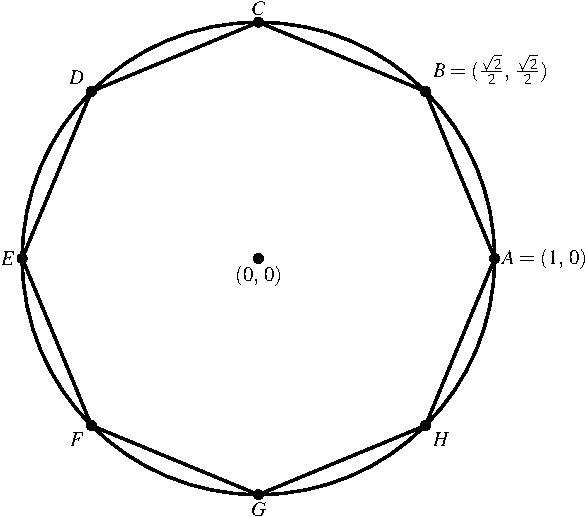
\includegraphics[scale=1.1]{image/05/circle-octagon.pdf}
\caption{%%
  A unit circle centred at the origin and having an inscribed
  octagon.  Except for the origin $\tuple{0}{0}$, the indicated points
  are where the octagon touches the unit circle.  Any two neighbouring
  points are $\degree{45}$~(or $\pi / 4$ radians) apart.
}
\label{fig:circle_inscribed_octagon}
\end{figure}

\Figure{fig:circle_inscribed_octagon} shows an octagon drawn inside a
unit circle.  Except for the origin $\tuple{0}{0}$, the eight labelled
points on the circle are where the octagon touches the circle.  Note
that any two neighbouring points are separated by
\[
\frac{\pi}{2} \times \frac{1}{2}
=
\frac{\pi}{4}
\]
radians.  The length of each side of the octagon is the length of the
line segment $AB$.  The distance from $A$ to $B$ is
%%
\begin{align*}
\sqrt{
  \parenthesis*{\frac{\sqrt{2}}{2} - 0}^2
  +
  \parenthesis*{\frac{\sqrt{2}}{2} - 1}^2
}
&=
\sqrt{
  \parenthesis*{\frac{\sqrt{2}}{2}}^2
  +
  \parenthesis*{\frac{\sqrt{2}}{2} - \frac{2}{2}}^2
} \\[4pt]
&=
\sqrt{
  \parenthesis*{\frac{\sqrt{2}}{2}}^2
  +
  \parenthesis*{\frac{\sqrt{2} - 2}{2}}^2
} \\[4pt]
&=
\sqrt{
  \frac{2}{4}
  +
  \frac{(\sqrt{2} - 2)^2}{4}
} \\[4pt]
&=
\sqrt{
  \frac{2}{4}
  +
  \frac{6 - 4\sqrt{2}}{4}
} \\[4pt]
&=
\sqrt{
  \frac{
    2 + 6 - 4\sqrt{2}
  }{
    4
  }
} \\[4pt]
&=
\sqrt{
  \frac{
    8 - 4\sqrt{2}
  }{
    4
  }
} \\[4pt]
&=
\sqrt{
  \frac{
    4(2 - \sqrt{2})
  }{
    4
  }
} \\[4pt]
&=
\sqrt{
  2 - \sqrt{2}
}.
\end{align*}
%%
In other words, each side of the octagon has a length of
$\ell = \sqrt{2 - \sqrt{2}}$.  Since the octagon has eight sides, then
the octagon has a perimeter of $8\ell = 8\sqrt{2 - \sqrt{2}}$ and you
can take this value to be an approximation of the circumference of the
unit circle.  Use \Equation{eqn:define_pi_as_ratio_of_c_over_d} to see
that the value of $\pi$ can be approximated as
%%
\begin{align*}
\pi
&\approx
\frac{
  8\sqrt{2 - \sqrt{2}}
}{
  2
} \\[4pt]
&\approx
4\sqrt{2 - \sqrt{2}} \\[4pt]
&\approx
3.061467
\end{align*}
%%
correct to six decimal places.  This is better than the
approximation~\eqref{eqn:approximate_pi_inscribed_square}, but is
worst than $22 / 7$.  You need to further decrease the angle that
separates two neighbouring points.


%%%%%%%%%%%%%%%%%%%%%%%%%%%%%%%%%%%%%%%%%%%%%%%%%%%%%%%%%%%%%%%%%%%%%%%%%%%

\section*{Problem}

\begin{problem}
\item You draw a pentagon inside the unit circle such that each of the
  five corners of the pentagon touches the unit circle.
  %%
  \begin{packedenum}
  \item Determine the coordinates of each of the five points of the
    pentagon.
  \end{packedenum}

\item A common formula for the area of a triangle is $\frac{1}{2} bh$,
  where $b$ is the length of the base of the triangle and $h$ is the
  triangle's height.  Another formula to calculate the area is
  \emph{Heron's formula}.  Heron's formula requires you to know the
  length of each side of the triangle.  Suppose that
  $\triple{a}{b}{c}$ are the lengths of the three sides of a triangle.
  Then the area of the triangle is
  \[
  \sqrt{
    s (s - a) (s - b) (s - c)
  }
  \]
  where $s$ is the fraction
  \[
  s
  =
  \frac{a + b + c}{2}.
  \]
  Let $O = \tuple{0}{0}$ be the origin.  In
  \Figure{fig:circle_inscribed_octagon}, compute the area of the
  triangle whose three corners are $\triple{O}{A}{B}$.
\ifbool{showSolution}{
\begin{solution}
The line segment $AB$ has a length of $\sqrt{2 - \sqrt{2}}$.  Since
each of the points $A$ and $B$ lie on a unit circle, the distance from
$A$ to the origin~(and the distance from $B$ to the origin) is the
radius of the circle, which is $1$.  In other words, each of the line
segments $AO$ and $BO$ has a length of $1$.  Write
%%
\begin{align*}
s
&=
\frac{
  1 + 1 + \sqrt{2 - \sqrt{2}}
}{
  2
} \\[4pt]
&=
\frac{
  2 + \sqrt{2 - \sqrt{2}}
}{
  2
}.
\end{align*}
%%
Use Heron's formula to see that the triangle with corners
$\triple{O}{A}{B}$ has an area of
\[
\sqrt{
  s (s - 1) (s - 1) \parenthesis*{s - \sqrt{2 - \sqrt{2}}}
}
=
\frac{\sqrt{2}}{4}.
\]
\end{solution}
}{}
\end{problem}

\end{document}
